\documentclass[12pt,a4paper]{report}

\usepackage[french]{babel}
\usepackage[utf8]{inputenc}
\usepackage[T1]{fontenc}
\usepackage{geometry}
\usepackage{graphicx}
\usepackage{listings}
\usepackage{xcolor}
\usepackage[hidelinks]{hyperref}

\geometry{margin=2.0cm}

\definecolor{codegreen}{rgb}{0,0.6,0}
\definecolor{codegray}{rgb}{0.5,0.5,0.5}

\lstset{
language=C,
extendedchars=true,
inputencoding=utf8,
basicstyle=\ttfamily\small,
keywordstyle=\color{blue},
commentstyle=\color{codegreen},
numbers=left,
numberstyle=\tiny\color{codegray},
breaklines=true,
frame=single,
showstringspaces=false,
showspaces=false, 
showtabs=false, 
% Ajout du support des accents français dans le code :
literate=
{é}{{\'e}}1
{è}{{\`e}}1
{à}{{\`a}}1
{ù}{{\`u}}1
{ç}{{\c{c}}}1
{É}{{\'E}}1
{È}{{\`E}}1
}
\begin{document}

\begin{titlepage}
\begin{center}
    \textbf{\Large REPUBLIQUE DU SENEGAL}
    
    \vspace{0.5cm}
    
\includegraphics{drapeau.png}
    
    \textbf{Un peuple - un but - une foi}   
      
    
    
    \vspace{0.5cm}
    \textbf{MINISTERE DE L'ENSEIGNEMENT SUPERIEUR DE LA RECHERCHE ET DE L'INNOVATION}
    \vspace{1cm}
    
    \textbf{\Large Université Iba Der Thiam de Thiès}
    
    
    
\includegraphics[height=5cm]{logo_uidt.png}
    
    \textbf{\Large Licence 2 Mathématiques et Informatique}
    
    \vspace{2cm}
    
    {\huge \textbf{RAPPORT DE PROJET}}
    
    \vspace{0.5cm}
    
    {\Large Annuaire d'une Fédération Sportive}
    
\end{center}

\textbf{\large Présenté et réalisé par :} \hspace{5cm} \textbf{\large Sous la direction de :} \\
  \large Mamadou Malal Diallo   \hspace{7cm}         \large Dr Abdoulaye Diallo

\vspace{4.2cm}
\centering{ \Large Année académique : 2025 - 2026}
	
    
\end{titlepage}
\tableofcontents
\newpage

\chapter*{Résumé}
\addcontentsline{toc}{chapter}{Résumé}

Dans le cadre du module Algorithmique et Structures de Données, nous avons développé une application de gestion d'une fédération sportive.  
Dans le cadre du module Algorithmique et Structures de Données, nous avons réalisé une application de gestion d'un annuaire de fédération sportive en langage C.

Cette application permet de gérer les clubs, les joueurs et les compétitions affiliés à une fédération sportive. Elle offre différentes fonctionnalités telles que l'ajout, la modification, la suppression, la recherche et le tri des données.

L'objectif principal est de mettre en pratique les notions de structures de données, de tableaux dynamiques, d'algorithmes de recherche et de tri, ainsi que la programmation modulaire en langage C.

\chapter{Introduction}
Le développement des systèmes informatiques a considérablement amélioré la gestion des organisations sportives. Les fédérations sportives doivent gérer un grand volume d'informations concernant les clubs, les joueurs et les compétitions.

La gestion manuelle de ces informations peut entraîner des erreurs, des pertes de données et un manque d'efficacité.

Pour répondre à ce besoin, nous avons développé une application permettant de centraliser et d'organiser toutes les informations relatives à une fédération sportive.

Les objectifs du projet sont :

\begin{itemize}
	\item Gérer les clubs sportifs.
	\item Gérer les joueurs.
	\item Gérer les compétitions.
	\item Faciliter les recherches, les tri et les mises à jour.
	\item Mettre en pratique les concepts d'algorithmique et de structures de données.
\end{itemize}

\chapter{Architecture}
\section{Vue d'ensemble}
L'application repose sur une architecture modulaire en couches :
\begin{itemize}
\item Couche métier : structures de données (joueurs, clubs, compétitions)
\item Couche logique : modules spécialisés (joueur.c, club.c, competition.c)
\item Couche présentation : interface utilisateur (main.c)
\item Couche utilitaire : fonctions utilitaires (util.c)
\end{itemize}	
\section{Structures de données et organisation mémoire}
\subsection{Structure Date}
\begin{lstlisting}
	/*=====================================================
	Structure date
	======================================================*/
	
	typedef struct {
		int jour; int mois; int annee;
	} Date;
\end{lstlisting}
\subsection{Structure Adresse}
\begin{lstlisting}
	typedef struct {
	    char siege[20], email[30], site_web[40], nom_stade[30], adresse_stade[20];
	} Adresse;
\end{lstlisting}
\subsection{Structure Joueur}
\begin{lstlisting}[language=C]	
	/*=====================================================
	Structure joueur
	======================================================*/
	typedef struct {
		char id[15];
		char prenom[40], nom[40];
		Date dateNaissance;
		char nationalite[40];
		char categorie[15];
		char poste[30];    
		char clubActuel[40];
		
	} Joueur;
\end{lstlisting}
\subsection{Structure Club}
\begin{lstlisting}[language=C]
	/*=====================================================
	Structure club
	======================================================*/
	typedef struct {
		char id[15];
		char nom[40];
		Date dateCreation;
		Adresse adresse;
		int points;
		char proprietaire[20], manager[20];
		int nb_pensionnaires, nb_pensionnaires_ajoutes;
		Joueur *pensionnaires;
	} Club;
\end{lstlisting}
Chaque club dispose d'un pointeur vers ses joueurs. 
\subsection{Structure Competition}
\begin{lstlisting}[language=C]
	/*=====================================================
	Structure competition
	======================================================*/
	typedef struct {
		char id[15];    
		char nom[40];
		char saison[10], type[40];
		int nb_max_paticipants;
		int nb_participants_ajoutes;
		Club *classement;
		Club *participants;
	} Competition;
\end{lstlisting}
Chaque compétition dispose d'un pointeur vers ses participants (clubs).
\subsection{Allocation dynamique}
Au démarrage, l'application invite l'utilisateur à configurer le système. La configuration consiste à spécifier les capacités maximales des jeux de données (joueurs, clubs, competitons). L'utilisateur devra saisir des valeurs entières. Tant que la valeur saisie n'est pas entière, un message d'erreur lui sera notifié et il sera encore invité à saisir une valeur entière. 
L'application alloue ainsi des tableaux dynamiques qui sont par la suite immuables.

\begin{lstlisting}[language=C]

	joueurs = (Joueur *)malloc(nb_joueurs_max * sizeof(Joueur));
	clubs = (Club *)malloc(nb_max_clubs * sizeof(Club));
	competitions = (Competition *)malloc(nb_max_competitions * sizeof(Competition));
\end{lstlisting}

Après la configuration du système, l'application affiche le menu principal. 
	

\section{Gestion de la mémoire dynamique}
Chaque ajout d'un objet (joueur, club, compétition) déclenche une vérification des capacités. Si la capacité maximale est atteinte alors une réallocation sera tentée par l'application, si elle échoue alors il ne sera pas possible d'effectuer l'ajout.
\begin{lstlisting}
	if (nb_joueurs_ajoutes >= nb_joueurs_max) {
		Joueur *temp = realloc(joueurs, (nb_joueurs_max + 1) * sizeof(Joueur));
		if (temp == NULL) {
			printf("                                            Nombre maximal de joueurs atteint (Echec de l'allocation mémoire).\n");
			return;
		}
		joueurs = temp;
		nb_joueurs_max++;
	}
\end{lstlisting}

\begin{lstlisting}
	if (nb_clubs_ajoutes >= nb_max_clubs)
	{
		Club *temp = realloc(clubs, (nb_max_clubs + 1) * sizeof(Club));
		if (temp == NULL){
			printf("                                            Nombre maximal de clubs atteint (Echec de l'allocation mémoire).\n");
			return;
		}
		clubs = temp;
		nb_max_clubs++;
	}
\end{lstlisting}

\begin{lstlisting}
	if (nb_competitions_ajoutes >= nb_max_competitions) {
		Competition *temp = realloc(competitions, (nb_max_competitions + 1) * sizeof(Competition));
		if (temp == NULL) {
			printf("                                            Nombre maximal de compétitions atteint (Echec de l'allocation mémoire).\n");
			return;
		}
		competitions = temp;
		nb_max_competitions++;
		
	}
\end{lstlisting}

\chapter{Les fonctionnalités}
L'application propose plusieurs fonctionnalités réparties dans cinq (5) menus.

\begin{itemize}
	\item 1- Menu joueurs
	\item 2- Menu clubs
	\item 3- Menu compétitions
	\item 4- Aller à l'accueil
	\item 5- QUITTER
\end{itemize}
\section{Menu joueurs}
Ce menu permet de gérer les joueurs. Ses fonctionnalités sont assurées par les fonctions implémentées dans le module joueur.c. Il propose 7 fonctionnalités.

\subsection{Ajouter un joueur}
Cette option permet d'ajouter un joueur. 
Tout d'abord l'application vérifie que la taille maximale spécifiée lors de la configuration n'est pas atteinte. Si elle atteinte l'ajout ne pourra pas se faire. Sinon l'utilisateur sera invité à remplir les champs du joueur. L'application s'assure que l'identifiant de chaque joueur soit unique pour éviter ainsi les doublons.
Lorsque l'utilisateur termine de remplir les champs, le joueur sera ajouté dans le tableau joueurs.
\begin{lstlisting}
	
	
	if (nb_joueurs_ajoutes >= nb_joueurs_max) {
		printf("Nombre maximal de joueurs atteint. Impossible d'ajouter plus de joueurs.\n");
		return;
	}
	int exist; char id[15];    
	do
	{   
		exist = 0;
		printf("Entrer l'identifiant du joueur : ");
		scanf(" %[^\n]", id);
		for (int i = 0; i < nb_joueurs_ajoutes; i++)
		{
			if(strcmp(joueurs[i].id, id) == 0){
				exist = 1;
				printf("\n                                            Cet identifiant existe déja.\n");
				break;
			}
		}               
	} while (exist);
	
	strcpy((joueurs+nb_joueurs_ajoutes)->id, id);    
	printf(" Entrer le prénom du joueur : ");
	scanf(" %[^\n]", (joueurs+nb_joueurs_ajoutes)->prenom); 
	printf("Entrer le nom du joueur : ");
	scanf(" %[^\n]", (joueurs+nb_joueurs_ajoutes)->nom); 
	printf("Entrer la date de naissance du joueur (jj mm aaaa) : ");
	scanf(" %d %d %d", &(joueurs+nb_joueurs_ajoutes)->dateNaissance.jour, 
	&(joueurs+nb_joueurs_ajoutes)->dateNaissance.mois, 
	&(joueurs+nb_joueurs_ajoutes)->dateNaissance.annee); 
	printf("Entrer la nationalité du joueur : ");
	scanf(" %[^\n]", (joueurs+nb_joueurs_ajoutes)->nationalite); 
	printf("Entrer la catégorie du joueur : ");
	scanf(" %[^\n]", (joueurs+nb_joueurs_ajoutes)->categorie); 
	printf("Entrer le poste du joueur : ");
	scanf(" %[^\n]", (joueurs+nb_joueurs_ajoutes)->poste);
	printf("Entrer le club actuel du joueur : ");
	scanf(" %[^\n]", (joueurs+nb_joueurs_ajoutes)->clubActuel);  
	puts("\n");  
	printf("%s %s a été ajouté avec succès !\n", (joueurs+nb_joueurs_ajoutes)->prenom, (joueurs+nb_joueurs_ajoutes)->nom);
	nb_joueurs_ajoutes++; 
\end{lstlisting}

\subsection{Afficher tous les joueurs}
Cette fonctionnalité permet d'afficher tous les joueurs enregistrés à l'aide de la fonction liste\_joueurs().
Si aucun joueur n'est enregistré alors un message sera affiché pour notifier l'utilisateur. 

\begin{lstlisting}
	if (nb_joueurs_ajoutes == 0) {
		printf("                                            Liste vide. Aucun joueur à afficher.\n");
		return;
	}
\end{lstlisting} 
S'il y a au moins un joueur enregistré alors ses informations seront affichées.

\subsection{Rechercher un joueur}
Cette fonctionnalité permet de rechercher un joueur à l'aide de la fonction rechercher\_joueur().

L'application vérifie en premier lieu si le tableau joueurs n'est pas vide, si c'est le cas un message d'erreur est affiché et l'application quitte immédiatement cette option.
Autrement, l'utilisateur saisit l'identifiant du joueur qu'il souhaite rechercher. Si un joueur avec cet identifiant est enregistré alors ses informations seront affichées. Sinon un message d'erreur sera notifié à l'utilisateur.

\subsection{Supprimer un joueur}
La fonctionnalité de cette option est assurée par la fonction supprimer\_joueur(). 

L'application vérifie en premier lieu si le tableau joueurs n'est pas vide, si c'est le cas un message d'erreur est affiché et l'application quitte immédiatement cette option.

Autrement, l'utilisateur saisit l'identifiant du joueur qu'il souhaite supprimer. Si un joueur avec cet identifiant est enregistré alors il sera supprimé du tableau joueurs. Sinon un message d'erreur sera notifié à l'utilisateur. 
La suppression se fait par décalage à gauche. Le nombre de joueurs est ainsi décrémenté.

\subsection{Mettre à jour un joueur}
Cette fonctionnalité permet de mettre à jour (modifier) un champ d'un joueur à l'aide de la fonction mise\_a\_jour\_joueur().

D'abord l'application s'assure qu'il y a au moins un joueur dans le tableau joueurs afin de tenter une modification et éviter d'utiliser le processeur inutilement.

S'il a un joueur dans le tableau joueurs alors l'utilisateur devra saisir l'identifiant du joueur qu'il souhaite modifier, puis l'application lancera une procédure de recherche du joueur ayant cet identifiant. Deux cas peuvent se présenter à l'issue de cette recherche.
\begin{itemize}
	\item Le joueur est retrouvé : dans ce cas l'utilisateur sera invité à choisir le champ qu'il souhaite modifié. Et la modification se fera instantanément.
	\item Le joueur ayant l'identifiant saisi n'est pas retrouvé : Dans ce cas un message d'erreur sera affiché signalant qu'aucun joueur n'est enregistré dans le tableau joueurs avec l'identifiant saisi.
\end{itemize}

\subsection{Trier les joueurs par id / nom}
Ces fonctionnalités permettent de trier les joueurs par id / nom à l'aide des fonctions trier\_joueurs\_par\_id() et trier\_joueurs\_par\_nom().

S'il y a un joueur dans le tableau joueurs alors il sera trié selon le choix de l'utilisateur. Sinon un message d'erreur sera affiché signalant que le tableau joueurs est vide. 

\section{Menu clubs}
Ce menu permet de gérer les clubs. Ses fonctionnalités sont assurées par les fonctions implémentées dans le module club.c. Il propose neuf (9) fonctionnalités.

\subsection{Ajouter un club}
Cette fonctionnalité permet d'ajouter un club dans le tableau clubs à l'aide de la fonction ajouter\_club().

L'application vérifie en premier lieu si le tableau clubs est apte à enregistrer un nouveau club. Si le tableau est déjà plein alors un message d'erreur sera affiché signalant que l'enregistrement ne pourra pas s'effectuer.

Autrement, l'utilisateur sera invité à saisir l'identifiant du club. L'application lancera alors une recherche afin de s'assurer que ce club n'est pas déjà enregistré dans le tableau joueurs afin d'éviter des doublons. L'application s'assure ainsi que l'identifiant de chaque club est unique. 
\begin{lstlisting}
	do
	{   
		exist = 0;
		printf("Entrer l'identifiant du club : ");
		scanf(" %[^\n]", id);
		for (int i = 0; i < nb_clubs_ajoutes; i++)
		{
			if(strcmp(clubs[i].id, id) == 0){
				exist = 1;
				printf("Cet identifiant existe déja.\n");
				break;
			}
		}               
	} while (exist);
\end{lstlisting}	
Après la saisie d'un identifiant acceptable, l'utilisateur pourra remplir les champs restants.

\subsection{Afficher tous les clubs}
Cette fonctionnalité permet d'afficher tous les clubs enregistrés dans le tableau clubs à l'aide de la fonction afficher\_club().

L'application affiche tous les joueurs enregistrés dans le tableau clubs si ce dernier n'est pas vide. Sinon il affichera un message d'erreur à la place.

\subsection{Rechercher un club}
Cette fonctionnalité permet de rechercher tous les clubs enregistrés dans le tableau clubs à l'aide de la fonction rechercher\_club().

Si le tableau clubs n'est pas vide alors l'utilisateur sera invité à saisir l'identifiant du club qu'il souhaite rechercher.
\begin{lstlisting}
	printf("\n Saisir l'identifiant du club recherché: ");    
	scanf(" %[^\n]", id);
\end{lstlisting}
Puis l'application effectuera la recherche dans le tableau clubs. Si un club ayant cet identifiant est retrouvé alors ses informations seront affichées sinon un message d'erreur sera affiché à la place. Si le tableau clubs est vide alors un message d'erreur sera affiché et l'application quittera immédiatement la fonction.
\begin{lstlisting}
	if (nb_clubs_ajoutes == 0) {
		printf("\n Aucun club enregistré.\n");
		return;
	}   
\end{lstlisting}

\subsection{Supprimer un club}
Cette fonctionnalité permet de supprimer un club du tableau clubs à l'aide de la fonction supprimer\_club().

Si le tableau clubs est vide alors l'application affiche un message d'erreur avant de quitter la fonction.
Sinon l'application invitera l'utilisateur à saisir l'identifiant du club qu'il souhaite supprimer. Le club ayant cet identifiant sera alors supprimé s'il est présent dans le tableau clubs ou bien un message d'erreur sera affiché à la place s'il y est absent.

\subsection{Mettre à jour un club}
Cette fonctionnalité permet de mettre à jour un champ d'un club enregistré dans le tableau club à l'aide de la fonction mise\_a\_jour\_club().

Si le tableau clubs est vide alors l'application affiche un message d'erreur avant de quitter la fonction. 
Sinon l'application invitera l'utilisateur à saisir l'identifiant du club qu'il souhaite modifier puis l'application lancera une procédure de recherche du club ayant cet identifiant. Deux cas peuvent se présenter à l'issue de cette recherche.
\begin{itemize}
	\item Le club est retrouvé : dans ce cas l'utilisateur sera invité à choisir le champ qu'il souhaite modifié. Et la modification se fera instantanément.
	\item Le club ayant l'identifiant saisi n'est pas retrouvé : Dans ce cas un message d'erreur sera affiché signalant qu'aucun club n'est enregistré dans le tableau clubs avec l'identifiant saisi.
\end{itemize}

\subsection{Trier les clubs par id et trier les clubs par nom}
Ces fonctionnalités permettent de trier le tableau clubs par id à l'aide de la fonction trier\_clubs\_par\_id() (tri par sélection) ou bien par nom à l'aide de la fonction trier\_clubs\_par\_nom() (tri à bulles).

Si le tableau clubs est vide alors l'application affiche un message d'erreur avant de quitter la fonction. Sinon le tableau sera trié selon le choix de l'utilisateur.

\subsection{Ajouter un joueur dans un club}
Cette fonctionnalité permet d'ajouter un joueur dans un club enregistré dans le tableau clubs à l'aide de la fonction ajouter\_joueur\_club().

Si le tableau clubs ou le tableau joueurs est vide alors l'application affiche un message d'erreur avant de quitter la fonction. 
\begin{lstlisting}
	if(nb_clubs_ajoutes == 0){
		printf("Aucun club enregistré\n"); 
		return;       
	}
	
	if(nb_joueurs_ajoutes == 0){
		printf("Aucun joueur enregistré\n");
		return;
	}
\end{lstlisting}
Si les conditions mentionnées ci-haut sont fausses alors l'utilisateur devra saisir l'identifiant du club auquel il souhaite ajouter un joueur. Après cette saisie, on distinguera deux cas :
\begin{itemize}
	\item Aucun club n'est enregistré dans le tableau clubs avec l'identifiant saisi. Dans ce cas l'application affiche un message d'erreur avant de quitter la fonction.
	\begin{lstlisting}
if(!club_trouve){
	printf("\n Aucun club enregistré avec cet identifiant\n", id_club);
}
	\end{lstlisting}
	\item Un club ayant cet identifiant est présent dans le tableau clubs. Dans ce cas l'utilisateur sera invité à saisir l'identifiant du joueur qu'il souhaite ajouter dans ce club. Après cette saisie, on distinguera trois résultats possibles :
	\begin{itemize}
		\item Le joueur ayant cet identifiant est déjà enregistré dans ce club. Alors l'application notifie l'utilisateur et quitte la fonction.
		\item Le joueur ayant cet identifiant est retrouvé dans le tableau joueurs mais n'est pas un joueur de ce club, dans ce cas le joueur sera automatiquement enregistré dans le tableau pensionnaires de ce club.
		\item Aucun joueur avec cet identifiant n'est enregistré dans le tableau joueurs, dans ce cas l'application affiche un message d'erreur avant de quitter la fonction. 
	\end{itemize}
\end{itemize}
\textbf{Remarque} : Le tableau pensionnaires est un tableau dynamique réalloué à chaque fois qu'il sera possible d'ajouter un joueur dans un club. Ceci permet d'éviter un gaspillage de l'espace mémoire du système.

\subsection{Afficher les joueurs d'un club}
Cette fonctionnalité permet d'afficher tous les joueurs d'un club enregistré dans le tableau clubs à l'aide de la fonction afficher\_joueur\_du\_club().\\
L'utilisateur sera invité à saisir l'identifiant du club dont il souhaite afficher les joueurs. Si ce club est présent dans le tableau clubs alors une liste de ses joueurs sera affichée (si le tableau pensionnaires de ce club n'est pas vide) sinon un message d'erreur sera affiché à la place.

\section{Menu compétitions}

Ce menu permet de gérer les compétitions. Ses fonctionnalités sont assurées par les fonctions implémentées dans le module competition.c. Il propose huit (8) fonctionnalités.
\subsection{Ajouter une compétition}
Cette fonctionnalité permet d'ajouter une compétition dans le tableau competitions à l'aide de la fonction ajouter\_competition().\\
L'application vérifie en premier lieu si le tableau competitions est apte à enregistrer une nouvelle compétition. Si le tableau est déjà plein alors un message d'erreur sera affiché signalant que l'enregistrement ne pourra pas s'effectuer.\\
Autrement, l'utilisateur sera invité à saisir un identifiant pour la compétition. L'application vérifie alors si l'identifiant saisi n'est pas déjà attribué à une compétition dans le tableau competitions. Si une compétition ayant cet identifiant est y déjà présent, alors l'utilisateur devra saisir un nouveau identifiant différent. Cela garantit l'unicité de l'identifiant de chaque compétition. Après cette opération, l'utilisateur pourra saisir les autres champs qui lui seront demandés.\\
A la fin des saisies, la compétition sera enregistré dans le tableau competitions.

\subsection{Ajouter des participants à une compétition}
Cette fonctionnalité permet d'ajouter un participant à une compétition à l'aide de la fonction ajouter\_participants().\\
L'application invite l'utilisateur à spécifier l'identifiant de la compétition dans laquelle il souhaite ajouter un participant (club). On distinguera alors deux cas : 
\begin{itemize}
	\item La compétition est enregistrée dans le tableau competition. Dans ce cas l'utilisateur sera invité à saisir l'identifiant du club qu'il souhaite ajouter dans cette compétition. Si ce club existe dans le tableau clubs alors il sera automatiquement ajouté dans le tableau participants de cette compétition s'il n'y est pas déjà présent. Sinon un message d'erreur sera affiché signalant l'inexistence d'un club ayant l'identifiant saisi pour le club.
	\item La compétition n'est pas enregistrée dans le tableau competition. Dans ce cas un message s'affichera signalant l'inexistence d'une compétition ayant l'identifiant saisi pour la compétition.
\end{itemize}
\textbf{Remarque} : Un même club ne peut être ajouté plus d'une fois dans une même compétition. Cela évite les doublons et respecte les critères d'une compétition sportive.

\subsection{Afficher les compétitions}
Cette fonctionnalité permet d'afficher toutes les compétitions enregistrées dans le tableau competitions à l'aide de la fonction afficher\_competition().\\
Si le tableau competitions est vide alors un message d'erreur s'affichera notifiant sur l'état de vacuité du tableau.
Autrement, une liste d'informations sur toutes les compétitions qui y sont enregistrées sera affichée.

\subsection{Rechercher une compétition} 
Cette fonctionnalité permet de rechercher une compétition enregistrée dans le tableau competitions, à l'aide de la fonction rechercher\_competition().\\
Si le tableau competitions est vide alors un message d'erreur sera affiché signalant l'état de vacuité du tableau. Autrement, l'utilisateur devra saisir l'identifiant de la compétition qu'il souhaite rechercher. On distinguera alors deux cas : 
\begin{itemize}
	\item La compétition recherchée est présente dans le tableau competitions, dans ce cas, ses informations seront affichées.
	\item La compétition recherchée est absente dans le tableau competitions, dans ce cas, un message d'erreur sera affiché pour notifier son absence. 
\end{itemize}
 
\subsection{Supprimer une compétition}
Cette fonctionnalité permet de supprimer une compétition du tableau competitions, à l'aide de la fonction supprimer\_competiton().\\
Si le tableau competitions est vide alors un message d'erreur sera affiché signalant l'état de vacuité du tableau. Autrement, l'utilisateur devra saisir l'identifiant de la compétition qu'il souhaite supprimer. On distinguera alors deux cas : 
\begin{itemize}
	\item Cette compétition est présente dans le tableau competitions, dans ce cas, elle sera supprimée du tableau.
	\item Cette compétition n'est pas présente dans le tableau competitions, dans ce cas, un message d'erreur sera affiché pour notifier son absence. 
\end{itemize} 

\subsection{Supprimer un participant}
Cette fonctionnalité permet de supprimer un participant (club) d'une compétition, à l'aide de la fonction supprimer\_participant().\\
Si le tableau competitions est vide alors un message d'erreur sera affiché signalant l'état de vacuité du tableau. Autrement, l'utilisateur devra saisir l'identifiant de la compétition où est enregistré le participant qu'il souhaite supprimer. On distinguera alors deux cas : 
\begin{itemize}
	\item Cette compétition est présente dans le tableau competitions, dans ce cas, il devra saisir l'identifiant du participant et s'il est présent dans le tableau participants de cette compétition alors il sera supprimé de ce tableau sinon un message d'erreur sera affiché notifiant son absence.
	\item Cette compétition n'est pas présente dans le tableau competitions, dans ce cas, un message d'erreur sera affiché pour notifier son absence. 
\end{itemize} 
\textbf{Remarque} : Si la compétition et le participant sont trouvés, alors le nombre de participants à cette compétition sera décrémenté après la suppression.

\subsection{Mettre à jour une compétition}
Cette fonctionnalité permet de modifier un ou des champs d'une compétition à l'aide de la fonction mise\_a\_jour\_competition().\\

\subsection{Trier les participants d'une compétition}
Cette fonctionnalité permet de trier les participants d'une compétition selon leur nombre de points dans l'ordre décroissant, à l'aide de la fonction trier\_participants().

\section{Aller à l'accueil}
Ce menu affiche la page de présentation de l'application. Il donne des informations sur le développeur de l'application et le nom du projet ayant donné naissance à l'application.

\section{Quitter}
Ce menu permet de quitter l'application définitivement.\\

\textbf{Remarque} : Une fois l'application quittée, toutes les données seront perdues.

\chapter{Etude de complexité} 
\section{Insertion}
L'insertion d'un enregistrement (joueur, club, compétition) suit le même schéma : \\
\begin{enumerate}
	\item Vérification que la capacité maximale n'est pas atteinte; 
	\item Vérification de l'unicité de l'identifiant par recherche séquentielle;
	\item Saisie interactive des champs via scanf ;
	\item Stockage à l'indice nb\_ajoutes et incrémentation du compteur.
\end{enumerate}
	La complexité est en $O(n)$ pour le contrôle d'unicité (recherche séquentielle).

 

\section{Recherche}
La recherche est effectuée par parcours séquentiel du tableau, avec comparaison des identifiants via strcmp. Si l'élément recherché est à la première position du tableau alors la complexité est $O(1)$ (dans le meilleur cas), s'il se trouve au milieu ou à la fin du tableau ou encore qu'il n'est pas dans le tableau alors la complexité est $O(n)$ (dans le moyen et pire cas).

\section{Suppression}
La suppression est réalisée par \textbf{décalage du tableau} : tous les éléments situés après la position supprimée sont décalés d'un rang vers la gauche.\\
la complexité est $O(n)$ pour cette opération.

\section{Mise à jour}
La mise à jour localise d'abord l'enregistrement par recherche séquentielle, puis propose un sous-menu permettant de modifier le champ souhaité. La complexité La complexité dépend alors de la recherche séquentielle.

\section{Algorithme de tri}
\subsection{Tri par sélection}
Le tri par sélection parcourt le tableau pour trouver l'élément minimum et l'échanger avec la position courante.\\
Complexité : $O(n^2)$ dans tous les cas.\\

\subsection{Tri à bulles}
Le tri à bulles compare des paires adjacentes et les échange si elles sont dans le mauvais
ordre.
Complexité : $O(n^2)$ dans tous les cas.

\section{Courbe de complexité}
Les fonctions de recherche et de tri ont été testées sur des tableaux statiques et des tableaux dynamiques afin de faire une étude comparative.
\subsection{Etude du tri par sélection}
Des expériences ont été réalisées dans des tableaux dynamiques et statiques manipulant les mêmes objets pour savoir lequel des deux types de tableaux est le plus favorable au tri par sélection.
Le graphique ci-dessous montrent les résultats obtenues à l'issue de ces expériences :\\ \\
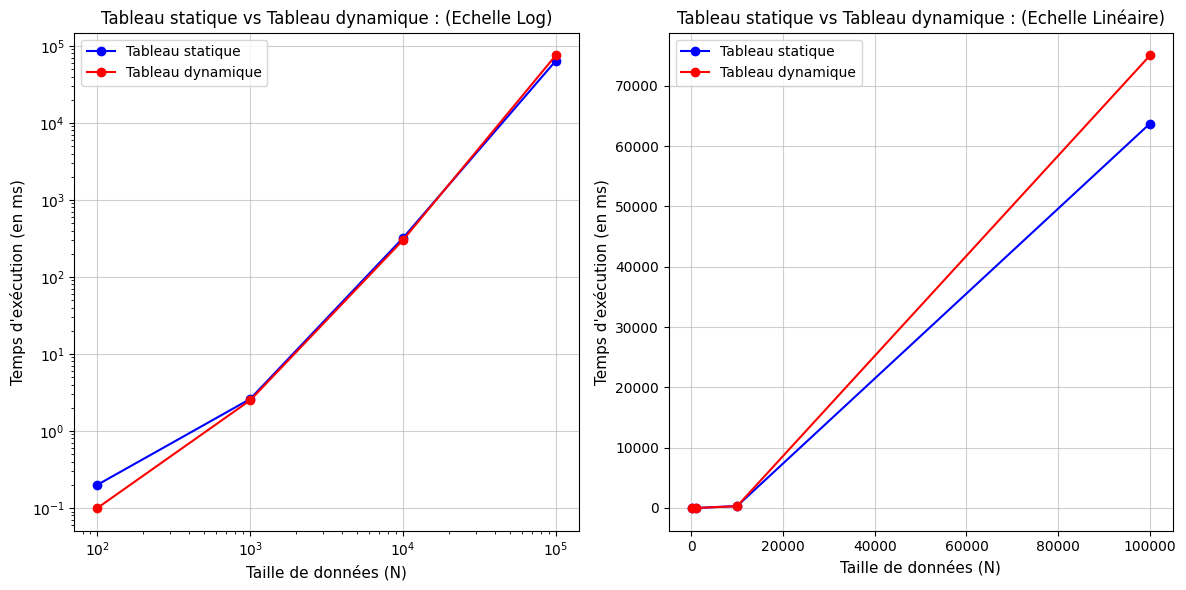
\includegraphics[width=19cm]{courbes_tri.png}
Soit N la taille des données.\\
D'après ce graphique, on constate que pour $N \in [10^2, 10^3]$, le tri par sélection dans un tableau dynamique est plus rapide que celui dans un tableau statique. Pour $N \in [10^3, 10^4]$, le coût du tri semble le même dans les deux tableaux. Et pour $N \in [10^4, 10^5]$, le tri est plus rapide dans un tableau statique que dans un tableau dynamique.
D'après ces observations, pour une quantité de données $N \leq 10^4$ l'utilisation d'un tableau dynamique est préférable pour le tri. Cependant pour une quantité de données $N \succ 10^4$, l'utilisation d'un tableau statique est le plus recommandé.

\subsection{Etude de la recherche séquentielle}
Des expériences ont été réalisées dans des tableaux dynamiques et statiques manipulant les mêmes objets pour savoir lequel des deux types de tableaux est le plus favorable à la recherche séquentielle.
Le graphique ci-dessous montrent les résultats obtenues à l'issue de ces expériences :\\ \\
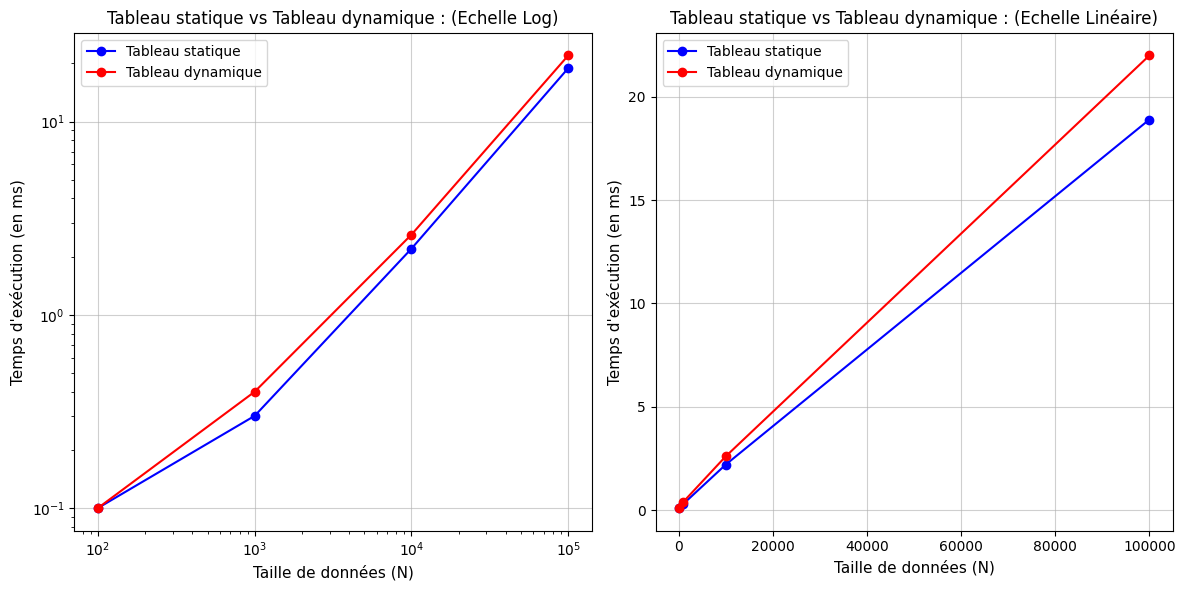
\includegraphics[width=19cm]{courbes_recherche.png} \\ \\
Soit N la taille des données.\\
D'après ce graphique, pour $N \in [100, 100000]$, la recherche est plus rapide dans un tableau statique que dans un tableau dynamique.\\
Donc pour la recherche séquentielle, il est préférable d'opter pour des tableaux statiques.

\chapter{Conclusion et perspectives}
\section{Bilan}
Ce projet a permis de mettre en pratique les concepts fondamentaux de l'algorithmique et des structures de données en langage C :
\begin{itemize}
	\item La conception de type enregistrements (struct) complexes et imbriqués avec des relations inter-entités réalisées par des pointeurs;
	\item L'implémentation des opérations classiques (insertion, suppression, recherche, tri) sur des tableaux alloués dynamiquement;
	\item L'analyse de complexité asymptotique des algorithmes mis en \oe{}uvre;
	\item La structuration du code en modules indépendants avec un Makefile fonctionnel;
	\item La production d'une interface utilisateur interactive en console.\\
\end{itemize}

Le domaine de l'annuaire de fédération sportive s'est avéré particulièrement adapté à ce projet, car il implique naturellement des entités hiérarchiques (fédération $\to$ compétitions $\to$ clubs $\to$ joueurs), favorisant l'utilisation de pointeurs et de tableaux dynamiques.

\section{Limites}
\begin{itemize}
	\item L'utilisation de \textbf{Windows.h}, \textbf{conio.h} et \textbf{Sleep()} rend le code non portable sur Linux/macOS;
	\item Toutes les données sont perdues à la fermeture de l'application;
	\item L'utilisateur revient toujours au menu principal après une opération; 
	\item Les caractères accentués ne sont pas acceptés dans les tableaux de caractères des enregistrements (Joueur, Club et Competition).
\end{itemize}
\section{Perspectives d'amélioration}
\begin{itemize}
	\item Ajouter une fonctionnalité permettant d'enregistrer les données dans un fichier et de les restaurer si besoin.
	\item Permettre la portabilité de l'application sur Linux/macOS;
	\item Liste doublement chaînée : alternative aux tableaux pour les insertions et suppressions fréquentes en milieu de collection ($O(1)$ après localisation);
	\item Forcer l'application à accepter les caractères accentués dans les tableaux de caractères des enregistrements (Joueur, Club et Competition).
\end{itemize}
Le lien suivant permet d'accéder au dépôt GitHub du projet : \\
\url{https://github.com/Malaldo/Annuaire_federation_sportive}

\end{document}